\documentclass[10pt]{article}  

%%%%%%%% PREÁMBULO %%%%%%%%%%%%
\title{Reporte de Laboratorio}
\usepackage{babel} %Indica que escribiermos en español
\usepackage[utf8]{inputenc} %Indica qué codificación se está usando ISO-8859-1(latin1)  o utf8  
\usepackage{amsmath} % Comandos extras para matemáticas (cajas para ecuaciones,
% etc)
\usepackage{amssymb} % Simbolos matematicos (por lo tanto)
\usepackage{longtable} %agregadom para hacer tablas
\usepackage{xltabular}
\usepackage{tabularray}
\usepackage{graphicx} % Incluir imágenes en LaTeX

\usepackage{color} % Para colorear texto
\definecolor{Blanco}{gray}{1}
\definecolor{Gray}{rgb}{0.501,0.501,0.501}
\definecolor{Tranquil}{rgb}{0.89,1,1}
\graphicspath{ {./images/} }

\usepackage{subfigure} % subfiguras
\usepackage{float} %Podemos usar el especificador [H] en las figuras para que se
% queden donde queramos
\usepackage{capt-of} % Permite usar etiquetas fuera de elementos flotantes
% (etiquetas de figuras)
\usepackage{sidecap} % Para poner el texto de las imágenes al lado
	\sidecaptionvpos{figure}{c} % Para que el texto se alinie al centro vertical
\usepackage{caption} % Para poder quitar numeracion de figuras
\usepackage{commath} % funcionalidades extras para diferenciales, integrales,
% etc (\od, \dif, etc)
\usepackage{cancel} % para cancelar expresiones (\cancelto{0}{x})
 
\usepackage{anysize} 					% Para personalizar el ancho de  los márgenes
\marginsize{2cm}{2cm}{2cm}{2cm} % Izquierda, derecha, arriba, abajo

\usepackage{appendix}
\renewcommand{\appendixname}{Apéndices}
\renewcommand{\appendixtocname}{Apéndices}
\renewcommand{\appendixpagename}{Apéndices} 
% Para que las referencias sean hipervínculos a las figuras o ecuaciones y
% aparezcan en color
\usepackage[colorlinks=true,plainpages=true,citecolor=blue,linkcolor=blue]{hyperref}
\usepackage{fancyhdr} 
\pagestyle{fancy}
\fancyhf{}
\fancyhead[L]{\footnotesize UNI} %encabezado izquierda
\fancyhead[R]{\footnotesize Fac. de Ciencias}   % dereecha
\fancyfoot[R]{\footnotesize Reporte}  % Pie derecha
\fancyfoot[C]{\thepage}  % centro
\fancyfoot[L]{\footnotesize Segunda Ley de Newton}  %izquierda
\renewcommand{\footrulewidth}{0.4pt}


\usepackage{listings} % Para usar código fuente
\definecolor{dkgreen}{rgb}{0,0.6,0} % Definimos colores para usar en el código
\definecolor{gray}{rgb}{0.5,0.5,0.5} 
% configuración para el lenguaje que queramos utilizar
\lstset{language=Matlab,
   keywords={break,case,catch,continue,else,elseif,end,for,function,
      global,if,otherwise,persistent,return,switch,try,while},
   basicstyle=\ttfamily,
   keywordstyle=\color{blue},
   commentstyle=\color{red},
   stringstyle=\color{dkgreen},
   numbers=left,
   numberstyle=\tiny\color{gray},
   stepnumber=1,
   numbersep=10pt,
   backgroundcolor=\color{white},
   tabsize=4,
   showspaces=false,
   showstringspaces=false}

\newcommand{\sen}{\operatorname{\sen}}	% Definimos el comando \sen para el seno
%en español

\title{Plantilla para Reportes IMEC-UTB}
% Basada en la plantilla para reportes UPIITA de  Overleaf

%%%%%%%% TERMINA PREÁMBULO %%%%%%%%%%%%

\begin{document}

%%%%%%%%%%%%%%%%%%%%%%%%%%%%%%%%%% PORTADA %%%%%%%%%%%%%%%%%%%%%%%%%%%%%%%%%%%%%%%%%%%%
																					%%%
\begin{center}																		%%%
\newcommand{\HRule}{\rule{\linewidth}{0.5mm}}									%%%\left
 																					%%%

\hspace{0.9cm}

\textsc{\huge Universidad Nacional de Ingeniería }\\[0.8cm]
			
\textsc{\LARGE Facultad de Ciencias}

\vspace{0.6cm}



\includegraphics[scale = 0.15]{UNI.png}

													 								%%%
\vspace*{0.6cm}								%%%
																					%%%	



\begin{minipage}{0.9\textwidth} 
\begin{center}																					%%%
\textsc{\LARGE  Laboratorio de Física BFI01 A}
\end{center}
\end{minipage}\\[0.3cm]
%%%
    																				%%%
 			\vspace*{0.4cm}																		%%%
																					%%%
\HRule \\[0.5cm]																	%%%
{ \huge \bfseries Segunda Ley de Newton}\\[0.2cm]	%%%
 																					%%%
\HRule \\[0.9cm]																	%%%
 																				%%%
																					%%%
\begin{minipage}{0.46\textwidth}													%%%
\begin{flushleft} \large															%%%

% Aqui a continuación pongan los nombres de los integrantes
\emph{El grupo conformado por:}\\[2mm]
Llactahuaman Quispe Benjamin\\20232268G \\[1mm]
Cortez Núñez Christian\\20232203B\\[1mm]
Rocca Cruz Axel\\20234046A\\[1mm]
 

%%%
			%\vspace*{2cm}	
            													%%%
										 						%%%
\end{flushleft}																		%%%
\end{minipage}		
																%%%
\begin{minipage}{0.52\textwidth}		
\vspace{-1.9cm}											%%%
\begin{flushright} \large															%%%
\emph{Profesor:}\\[2mm]																	%%%
Tello Gálvez Julio César\\[1mm]Brocca Pobes Manuel Enrique\\
\end{flushright}																	%%%
\end{minipage}	
\vspace*{1cm}
%\begin{flushleft}
 	
%\end{flushleft}
%%%																	%%%															
\vspace{-2.4cm}	
\begin{minipage}{0.98\textwidth}
\begin{flushright}	
\large
\emph{Fecha de la práctica:}\\
\vspace{0.2cm}
12 de mayo de 2023 
\end{flushright}
\end{minipage}

 \vspace{2.4cm}

\large{\today}\\
\vspace{0.3cm}

{ \Large\bfseries 2023-1}
										 			
\end{center}							 											
																					
\newpage																		
%%%%%%%%%%%%%%%%%%%% TERMINA PORTADA %%%%%%%%%%%%%%%%%%%%%%%%%%%%%%%%

\tableofcontents 

\newpage

\begin{center}
    \textbf{\huge Segunda Ley de Newton}
\end{center}

\section{Objetivos}
\subsection{Competencias Generales}
\begin{itemize}
    \item Verificar experimentalmente la segunda ley de Newton
\end{itemize} 
\subsection{Competencias Específicas}
\begin{itemize}
    \item Calibrar dos resortes para hallar su constante elástica y con ello hallar la fuerza que estos aplican sobre un disco.
    \item Hallar la aceleración a partir de los ticks marcados por el disco sobre el papel donde realiza su trayectoria.
\end{itemize}


\begin{itemize}
    \item El resorte A (de 10,1 cm) presentaba una deformación en uno de sus extremos, la cuál no se tomó en cuenta para la longitud inicial debido a que era un segmento prácticamente rígido.
    \item La deformación mostrada por ambos resortes con solo el primer peso era considerablemente menor que la incertidumbre de los instrumentos de medición.
    \item Debido a la distribución del tablero el punto B se ubicaba 1,4 cm por fuera del papel, lo que dificultó tomar las medidas para cada punto de la trayectoria.
    \item El chispero en el segmento más acentuado de la curva dejaba marcados dos puntos en lugar de uno por cada tick.
\end{itemize}

\section{Conclusiones}

\begin{itemize}
    \item Se logró verificar experimentalmente la segunda Ley de Newton. El valor promedio del cociente entre el módulo de la fuerza y aceleración es 2,206 Kg y la desviación estándar es 0,133 por lo cual se obtuvo un error mínimo en los resultados.
    \item Se logró calibrar los resortes A y B y se halló que sus constantes de elasticidad son 28,399 N/m y 35,102 N/m respectivamente.
\end{itemize}

\section*{1. Introducción y objetivos del experimento}
El presente informe se basa en los datos recopilados de la experimentación en el laboratorio de Física II, en la Facultad de Ciencias. Se apoya en la guía de laboratorio y otras fuentes detalladas más adelante. El propósito del informe es responder las preguntas del cuestionario, de manera adecuada; así como contrastar los resultados de la experimentación con el fundamento teórico. De acuerdo a la guía del laboratorio e indicaciones del profesor, se ha dividido el informe de la siguiente manera.

\subsection*{1.1. Contenido}
\begin{enumerate}
  \item Introducción y objetivos del experimento
\end{enumerate}

\begin{itemize}
  \item Contenido
  \item Competencias generales
  \item Competencias específicas
\end{itemize}

\begin{enumerate}
  \setcounter{enumi}{1}
  \item Fundamento teórico
\end{enumerate}

\begin{itemize}
  \item Energía cinética de rotación y traslación
  \item Momento de inercia
  \item Dinámica de cuerpo rígido
  \item Movimiento de rodadura
  \item Aplicaciones en el experimento
\end{itemize}

\begin{enumerate}
  \setcounter{enumi}{2}
  \item Equipo utilizado y diagrama de flujo del experimento
\end{enumerate}

\begin{itemize}
  \item Equipo utilizado
  \item Diagrama de flujo del experimento
\end{itemize}

\begin{enumerate}
  \setcounter{enumi}{3}
  \item Procedimiento experimental
  \item Cálculos y resultados
\end{enumerate}

\begin{itemize}
  \item Uso de unidades
  \item Uso de cifras significativas
  \item Cálculo de errores
  \item Resultados obtenidos y comparación con otros conocidos
  \item Resultados obtenidos
  \item Tablas, gráficos y comparación con otros resultados conocidos
\end{itemize}

\begin{enumerate}
  \setcounter{enumi}{5}
  \item Cuestionario, observaciones y sugerencias
\end{enumerate}

\begin{itemize}
  \item Respuestas al cuestionario
  \item Observaciones
  \item Sugerencias
\end{itemize}

\begin{enumerate}
  \setcounter{enumi}{6}
  \item Conclusiones
  \item Bibliografía
\end{enumerate}

\subsection*{1.2. Competencias generales}
\begin{itemize}
  \item Observar el movimiento de rodadura de una rueda de Maxwell y a partir de las mediciones efectuadas determinar el momento de inercia de la rueda con respecto al eje perpendicular que pasa por su centro de su gravedad.
\end{itemize}

\subsection*{1.3. Competencias específicas}
\begin{itemize}
  \item Medir el tiempo en el cual la rueda realiza cada recorrido.
  \item Medir la masa y dimensiones de la rueda para calcular el momento de inercia de la rueda por dos métodos: Por su energía cinética de rotación y por la distribución geométrica de su masa.\\
*Aclaración: Debido a indicaciones del profesor, no se calculó el momento de inercia de la rueda por la distribución geométrica de su masa.
\end{itemize}

\section*{2. Fundamento teórico}
\subsection*{2.1. Energía cinética de rotación y traslación}
Sabemos que la energía cinética viene dada por la expresión $E_{c}=\frac{1}{2} m v^{2}$.\\
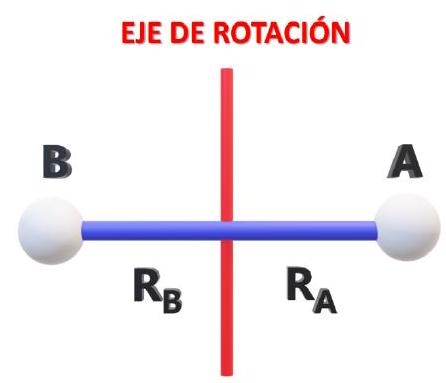
\includegraphics[scale = 0.15, center]{2025_04_01_ea720b93e8ebb5d0c6aeg-03}

Figura 1: Sistema simple\\
Considerando el sistema de dos cuerpos A y B unidos por una barra de masa insignificante que rotan alrededor de un eje que pasa por un punto de la barra y es\\
perpendicular a esta con velocidad angular $\vec{w}$, mostrado en 1 ; luego, la energía cinética del sistema está dada por la siguiente expresión:


\begin{equation*}
E_{c}(\text { sistema })=\frac{1}{2} m_{A} v_{A}^{2}+\frac{1}{2} m_{B} v_{B}^{2} \tag{1}
\end{equation*}


Pero tenemos: $\left|\overrightarrow{v_{A}}\right|=v_{A}=|\vec{w}|\left|\overrightarrow{R_{A}}\right|=w R_{A}$ y $\left|\overrightarrow{v_{B}}\right|=v_{B}=|\vec{w}|\left|\overrightarrow{R_{B}}\right|=w R_{B}$. Reemplazando en 1:


\begin{equation*}
E_{c}(\text { sistema })=\frac{1}{2} m_{A} w^{2} R_{A}^{2}+\frac{1}{2} m_{B} w^{2} R_{B}^{2} \tag{2}
\end{equation*}


Vemos que, en el caso de la rotación, la energía cinética depende del eje elegido, por lo que debemos separar la energía cinética en el movimiento de traslación y rotación. Luego $E_{\text {rotacionalA }}=\frac{1}{2} m_{A} w^{2} R_{A}^{2}$ y $E_{\text {rotacional } B}=\frac{1}{2} m_{B} w^{2} R_{B}^{2}$

\subsection*{2.2. Momento de inercia}
De 2 podemos factorizar $\frac{1}{2} w^{2}$.

$$
\begin{aligned}
E_{c}(\text { sistema }) & =\frac{1}{2} m_{A} w^{2} R_{A}^{2}+\frac{1}{2} m_{B} w^{2} R_{B}^{2} \\
& =\frac{1}{2}\left(m_{A} R_{A}^{2}+m_{B} R_{B}^{2}\right) w^{2} \\
& =\frac{1}{2} I w^{2}
\end{aligned}
$$

De donde definimos $I=m_{A} R_{A}^{2}+m_{B} R_{B}^{2}$ como el momento de inercia del sistema respecto al eje, con $R_{A}$ y $R_{B}$ las distancias de los cuerpos A y B al eje, respectivamente. Entonces si tenemos un sistema discreto de "n"partículas, el momento de inercia respecto a un eje está dado por la siguiente expresión:


\begin{equation*}
\sum_{i=1}^{n} m_{i} R_{i}^{2} \tag{3}
\end{equation*}


Donde $m_{i}$ es la masa del cuerpo i-ésimo y $R_{i}$ es la mínima distancia del cuerpo i-ésimo al eje de rotación. Luego, si tenemos un sistema de masas continuo, debemos realizar esta sumatoria en base a un diferencial de masa $(d m \rightarrow 0)$ con distancia mínima $r_{i}$ al eje de rotación.


\begin{equation*}
I=\lim _{d m_{i} \rightarrow 0} \sum r_{i}^{2} d m_{i} \tag{4}
\end{equation*}


Esto resulta ser la integral:


\begin{equation*}
I=\int r^{2} d m \tag{5}
\end{equation*}


Para resolver esta integral, hace falta saber como varía la masa respecto a la distancia mínima al eje de rotación.\\
Si ya conocemos el centro de masa del objeto, y consideramos una lámina plana de este, podemos hallar el momento de inercia de un eje paralelo a uno que pase por el centro de masa del objeto y que sea perpendicular al plano de la lámina.\\
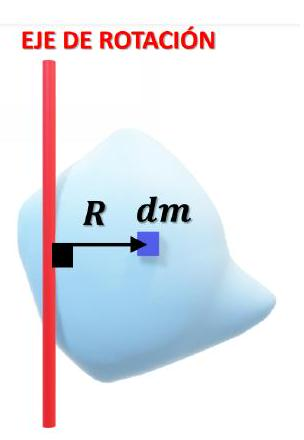
\includegraphics[scale = 0.15, center]{2025_04_01_ea720b93e8ebb5d0c6aeg-05}

Figura 2: Sistema de masas continuo\\
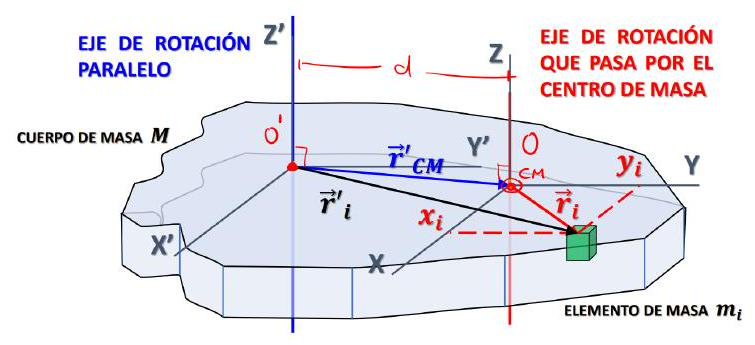
\includegraphics[scale = 0.15, center]{2025_04_01_ea720b93e8ebb5d0c6aeg-05(1)}

Figura 3: lámina plana del objeto.

Donde $\overrightarrow{r_{i}}$ es la posición del elemento de masa $m_{i}$ respecto al $\mathrm{CM},{\overrightarrow{r_{i}}}^{\prime}$ es la posición del elemento respecto al eje paralelo y $\overrightarrow{C M}^{\prime}$ es la posición del centro de masa respecto al eje paralelo.\\
Luego, sabemos que : $\vec{r}_{i}^{\prime}=r_{C M}^{\prime}+\overrightarrow{r_{i}}, \sum_{i=1}^{n} m_{i} r_{i}^{\prime 2},{\overrightarrow{r_{i}}}^{\prime}={\overrightarrow{x_{i}}}^{\prime}+\vec{y}_{i}^{\prime}$ con $x_{i} \perp y_{i}$. Luego:

$$
\begin{aligned}
\sum_{i=1}^{n} m_{i} r_{i}^{\prime 2} & =\sum_{i=1}^{n} m_{i}\left({\overrightarrow{x_{i}}}^{\prime}+\vec{y}_{i}^{\prime}\right)^{2} \\
& =\sum_{i=1}^{n} m_{i}\left(x_{i}^{\prime 2}+y_{i}^{\prime 2}\right) \\
& =\sum_{i=1}^{n} m_{i}\left(x_{C M}^{\prime}+\overrightarrow{x_{i}}\right)^{2}+\sum_{i=1}^{n} m_{i}\left(y_{\overrightarrow{C M}}{ }^{\prime}+\vec{y}_{i}\right)^{2}
\end{aligned}
$$

Donde :\\
$\sum_{i=1}^{n} m_{i}\left(x_{C M}^{\prime}+\vec{x}_{i}\right)^{2}=\sum_{i=1}^{n} m_{i} x_{C M}^{\prime 2}+2 \sum_{i=1}^{n} m_{i}<x_{C M}^{\prime}, \vec{x}_{i}>+\sum_{i=1}^{n} m_{i} x_{i}^{2}$\\
$\sum_{i=1}^{n} m_{i}\left(\overrightarrow{C M}^{\prime}+\overrightarrow{y_{i}}\right)^{2}=\sum_{i=1}^{n} m_{i} y_{C M}^{\prime 2}+2 \sum_{i=1}^{n} m_{i}<y_{\text {CM }^{\prime}}, \overrightarrow{y_{i}}>+\sum_{i=1}^{n} m_{i} y_{i}^{2}$\\
Pero sabemos que $x_{\overrightarrow{C M}}{ }^{\prime}$ y $y_{\overrightarrow{C M}}{ }^{\prime}$ son constantes. entonces:

$$
\sum_{i=1}^{n} m_{i}<x_{\overrightarrow{C M}}{ }^{\prime}, \vec{x}_{i}>=<x_{C M}^{\prime}, \sum_{i=1}^{n} m_{i}{\overrightarrow{x_{i}}}^{\prime} y \sum_{i=1}^{n} m_{i}<y_{C M}{ }^{\prime}, \vec{y}_{i}>=<y_{C M}^{\prime}, \sum_{i=1}^{n} m_{i} \vec{y}_{i}>
$$

$$
\sum_{i=1}^{n} m_{i} \overrightarrow{x_{i}}=\sum_{i=1}^{n} m_{i}\left(\vec{x}_{i}^{\prime}-x_{C M}^{\prime}\right)=\overrightarrow{0}, \sum_{i=1}^{n} m_{i} \overrightarrow{y_{i}}=\sum_{i=1}^{n} m_{i}\left(\vec{y}_{i}^{\prime}-y_{C M}^{\prime}\right)=\overrightarrow{0}
$$

Entonces:

$$
\begin{aligned}
& \sum_{i=1}^{n} m_{i} r_{i}^{\prime 2}=\sum_{i=1}^{n} m_{i}\left(x_{C M}^{\prime 2}+y_{C M}^{\prime 2}\right)+\sum_{i=1}^{n} m_{i}\left(x_{i}^{2}+y_{i}^{2}\right) \\
& \text { Luego }: \\
& I_{\text {ejeparalelo }}=I_{C M}+M d^{2}
\end{aligned}
$$

Donde d es la distancia del eje paralelo al eje que pasa por el CM del sistema. Luego, esto se replica en todas las láminas que conforman el volumen del objeto, dando a entender que se cumple en objetos de cualquier dimensión.\\
Físicamente, el momento de inercia es la resistencia que ofrece el cuerpo a rotar sobre el eje elegido. También hay que tomar en cuenta al eje elegido, pues de este depende el momento de inercia, al variar las distancias respecto al eje si es que lo cambiamos.

\subsection*{2.3. Dinámica de cuerpo rígido}
Definimos al torque de una fuerza como una cantidad asociada a la capacidad de la fuerza, de alterar el estado de rotación de un cuerpo rígido.\\
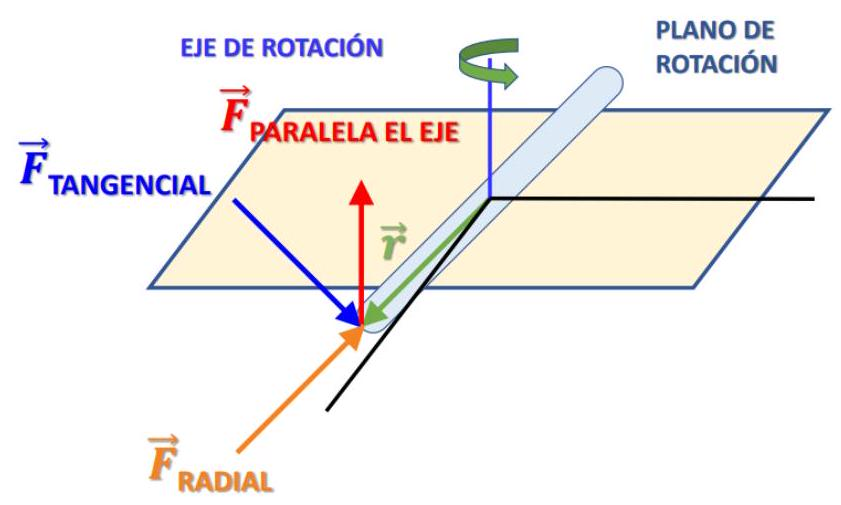
\includegraphics[scale = 0.15, center]{2025_04_01_ea720b93e8ebb5d0c6aeg-06}

Figura 4: Representación del torque de una fuerza

Observamos que solo $F_{\text {tangencial }}$ es capaz de alterar dicho estado de rotación respecto al punto de aplicación y el eje de rotación. Esto se debe a que, solo esta fuerza produce cambio en la velocidad tangencial y como $|\vec{v}|=|\vec{w}| \cdot|\vec{r}|$, implica entonces que $\vec{w}$ aumenta. Luego observamos que el sentido de giro está ligado a la dirección del vector $\vec{r} \times \vec{F}$. Luego afirmamos: ${\overrightarrow{t_{e j e}}}^{F}=\vec{r} \times \vec{F}$\\
Después, podemos notar que si la distancia respecto al eje de giro es lo suficientemente grande como para considerar al cuerpo rígido una partícula, podemos notar una nueva magnitud vectorial llamada momento angular, dada por la expresión $\vec{L}=\vec{r} \times \vec{p}$ (Donde\\
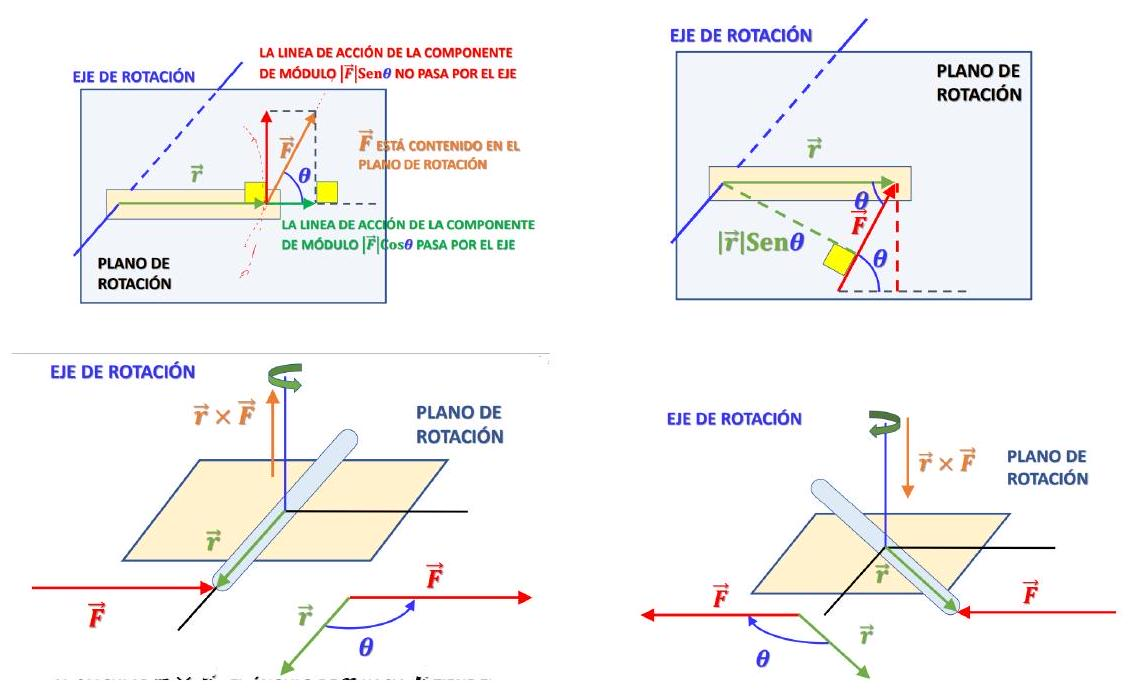
\includegraphics[scale = 0.15, center]{2025_04_01_ea720b93e8ebb5d0c6aeg-07(1)}

Figura 5: Representación de $\vec{r} \times \vec{F}$ y su relación con el torque\\
$p$ es la cantidad de movimiento lineal y r es la posición del cuerpo rígido respecto al eje de giro).\\
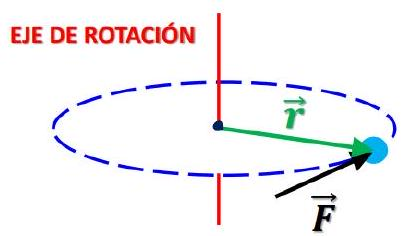
\includegraphics[scale = 0.15, center]{2025_04_01_ea720b93e8ebb5d0c6aeg-07}

Figura 6: Se desprecian las dimensiones del cuerpo rígido

Si derivamos $\vec{L}$ respecto al tiempo, tenemos:

$$
\begin{aligned}
\frac{d \vec{L}}{d t} & =\frac{d(\vec{r} \times \vec{p})}{d t} \\
& =\vec{r} \times \frac{d \vec{p}}{d t}+\frac{d \vec{r}}{d t} \times \vec{p} \\
& =\vec{r} \times \vec{F}+m \vec{v} \times \vec{v} \\
& =\vec{r} \times \vec{F} \\
& =\overrightarrow{t_{e j e}}
\end{aligned}
$$

Luego, si elegimos el eje adecuado, de tal manera que $\vec{L} \| \vec{w}$ (y al ocurrir: $\vec{r} \perp \vec{w}$ ). Tenemos: $\vec{L}=m \vec{r} \times(\vec{w} \times r)=m(<\vec{r}, \vec{r}>\vec{w}-<\vec{w}, \vec{r}>\vec{r})=m r^{2} \vec{w}=I \vec{w}$ Donde I es el momento de inercia del cuerpo rígido respecto al eje. Luego si derivamos, queda : $\overrightarrow{t_{e j e}^{F}}=I \vec{\alpha}$ (donde $\vec{\alpha}$ es la aceleración angular).

\subsection*{2.4. Movimiento de rodadura}
Un caso especial de la combinación del movimiento de traslación y rotación de un cuerpo rígido(en este caso una rueda simétrica), es el movimiento de rodadura pura(rueda sin resbalar). Físicamente, no resbalar significa que el punto de contacto entre\\
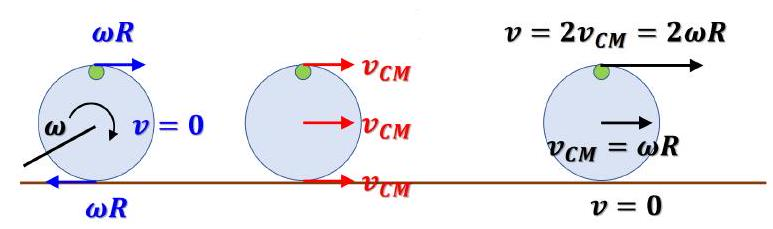
\includegraphics[scale = 0.15, center]{2025_04_01_ea720b93e8ebb5d0c6aeg-08(1)}

Figura 7: Rotación+Traslación sin resbalar\\
la rueda y la superficie no tenga desplazamiento ni velocidad, como consecuencia de las condiciones iniciales: $v_{C M}=w R$; este punto es llamado centro instantáneo de rotación(CIR), ya que la rueda aparenta rotar en un eje instantáneo perpendicular al plano de la rueda que pasa por el punto de contacto. De esto, tenemos que la rueda solo realiza rotación respecto al CIR, por lo que si hay pérdidas, estas serían por rotación y no por traslación. Pero observamos que podemos reformular la expresión en función a las características del centro de masa(velocidad de este y momento de inercia respecto a un eje que pasa por el centro de masa y es perpendicular al plano de la rueda).

$$
\begin{aligned}
E_{\text {rotacional }} & =\frac{1}{2} I_{C I R} w^{2} \\
& =\frac{1}{2}\left(I_{C M}+m R^{2}\right) w^{2} \\
& =\frac{1}{2} I_{C M} w^{2}+\frac{1}{2} m(w R)^{2} \\
& =\frac{1}{2} I_{C M} w^{2}+\frac{1}{2} m v_{C M}^{2} \\
& =E_{\text {rotacional } / C M}+E_{\text {traslacional } / C M}
\end{aligned}
$$

Donde $m$ es la masa de la rueda.\\
En el caso ideal, la rueda y la superficie no se deforman por acción de las fuerzas. Como\\
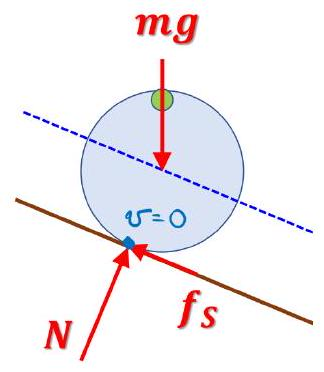
\includegraphics[scale = 0.15, center]{2025_04_01_ea720b93e8ebb5d0c6aeg-08}

Figura 8: DCL de la rueda en un plano inclinado.\\
el punto de contacto no se desplaza, $W_{f s}=W_{F N C}=0$ y por lo tanto se conserva la\\
energía mecánica.\\
En un caso real, se consideran las deformaciones de la rueda y la superficie, además se puede apreciar que la rueda desliza producto de las formaciones, este fenómeno se conoce como fricción por rodadura.\\
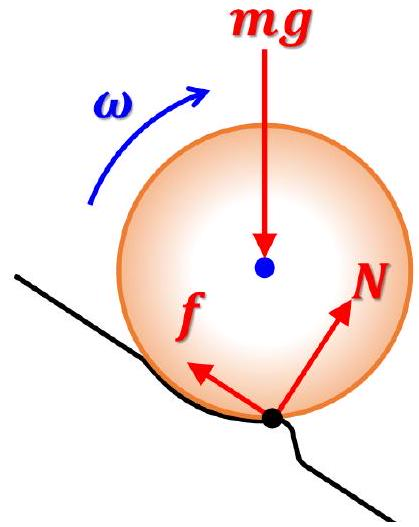
\includegraphics[scale = 0.15, center]{2025_04_01_ea720b93e8ebb5d0c6aeg-09}

Figura 9: Se aprecian deformaciones

Esto causa la pérdida de energía mecánica; aunque es común despreciar este efecto en experimentaciones reales, al ser la rueda y la superficie muy rígidas como para observar efectos apreciables a causa de la fricción por rodadura, por lo que consideramos, la energía mecánica se conserva en estos casos también.

\subsection*{2.5. Aplicaciones en el experimento}
Tenemos una rueda de Maxwell brindada en el laboratorio, que tiene un eje perpendicular al plano de la rueda, el cual pasa por su centro de gravedad. El eje es un cilindro concéntrico a la rueda con un radio $\mathrm{r}<\mathrm{R}$ (radio de la rueda), similar a lo que se muestra en la figura (a). En la figura 10b tenemos marcados los puntos $A_{0}, A_{1}, A_{2}$,\\
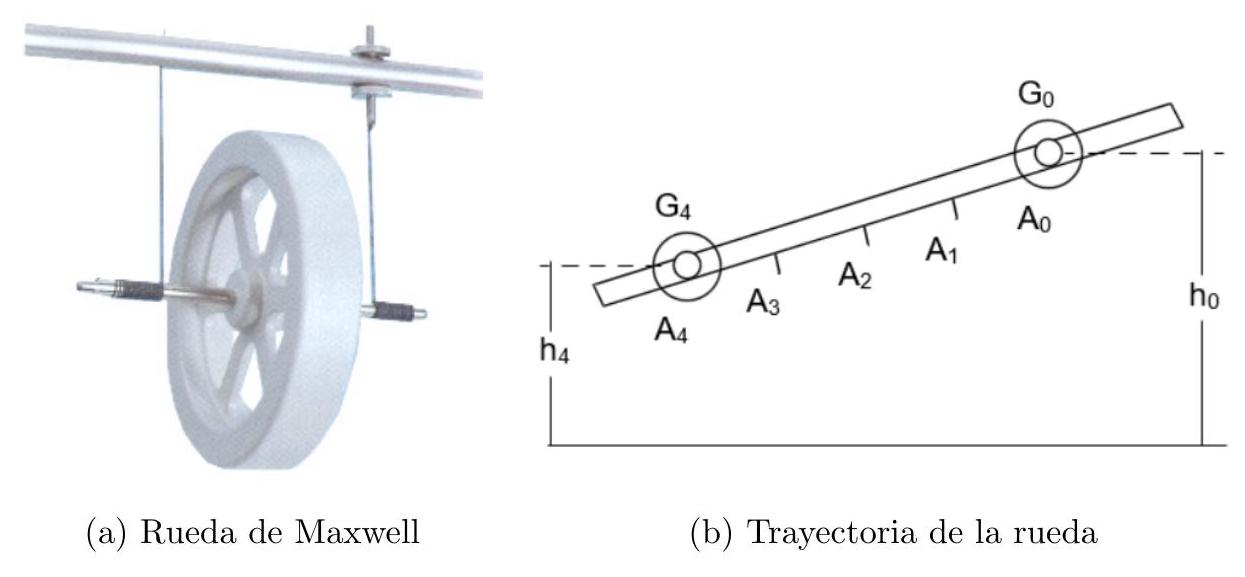
\includegraphics[scale = 0.15, center]{2025_04_01_ea720b93e8ebb5d0c6aeg-09(1)}

Figuras referenciales\\
$A_{3}$ y $A_{4}$ separados 10 cm ; tenemos también $G_{0}$ y $G_{4}$ que representan las posiciones del centro de gravedad de la tierra, en el punto más alto y bajo de su trayectoria respectivamente. Por todo lo antes visto, despreciamos la fricción por rodadura, y por ende, se conserva la energía mecánica. Por lo que :


\begin{align*}
E_{M(4)} & =m g h_{4}+\frac{1}{2} I_{G} w_{G_{4}}^{2}+\frac{1}{2} m v_{G_{4}}^{2}  \tag{6}\\
& =m g h_{4}+\frac{1}{2} I_{G} \frac{v_{G_{4}}^{2}}{r^{2}}+\frac{1}{2} m v_{G_{4}}^{2}  \tag{7}\\
& =E_{M(0)}  \tag{8}\\
& =m g h_{0}+\frac{1}{2} I_{G} \frac{v_{G_{0}}^{2}}{r^{2}}+\frac{1}{2} m v_{G_{0}}^{2}  \tag{9}\\
m g h_{0}\left(v_{G_{0}}=0\right) & =m g h_{4}+\frac{1}{2} I_{G} \frac{v_{G_{4}}^{2}}{r^{2}}+\frac{1}{2} m v_{G_{4}}^{2} \tag{10}
\end{align*}


Luego $x=\frac{1}{2} a t^{2}$ respecto al centro de gravedad al ser la posición inicial $x=0 \mathrm{y}$ observarse un MRUV por parte de la rueda, producto de una aceleración constante producida por el peso, la fricción estática y la fuerza normal. Luego sabemos $v_{G}=a t$ al ser $v_{0}=0$, luego $v_{G}=\frac{2 x}{t}$. Con todo esto, podemos realizar el experimento y verificar los resultados, midiendo solo la velocidad, el radio del eje de giro, el desplazamiento y el tiempo transcurrido.

\section*{3. Equipo utilizado y diagrama de flujo del experimento}
\subsection*{3.1. Equipo utilizado}
\begin{itemize}
  \item Un par de rieles paralelos (como plano inclinado)
  \item Una rueda de Maxwell
  \item Un cronómetro digital
  \item Un pie de rey
  \item Una regla milimetrada
  \item Una balanza
  \item Un nivelador
\end{itemize}


\end{document}
